\documentclass[11pt]{article}
\usepackage[utf8]{inputenc}
\usepackage[T1]{fontenc}
\usepackage{minted}
\usepackage{graphicx}
\usepackage{hyperref}
\usepackage{CJKutf8}

\author{Student: Brian Cheung bc32427 \\ Professor: Mohit Tiwari \\ TA: Antonio Espinoza \\ Department of Electrical \& Computer Engineering \\ The University of Texas at Austin}
\date{\today}
\title{EE379K Enterprise Network Security Lab 2 Report}
\hypersetup{
 pdfauthor={Student: Brian Cheung bc32427 \\ Professor: Mohit Tiwari \\ TA: Antonio Espinoza \\ Department of Electrical \& Computer Engineering \\ The University of Texas at Austin},
 pdftitle={EE379K Enterprise Network Security Lab 2 Report},
 pdfkeywords={},
 pdfsubject={},
 pdfcreator={},
 pdflang={English}}

\begin{document}

\maketitle
\newpage
\section*{Part 1 - Vulnerable Web Apps}
\label{sec:part-1}
\subsection*{1a - Set up a web-service in a container}
For this lab, the Damn Vulnerable Web App (DVWA) was set up as a web-service in a Docker container
using the following guide ~\cite{dvwa} and set to low difficulty.

\subsubsection*{PHP Injection}
The objective of this section was to implement a PHP injection that printed out the path to the current directory,
the contents of the current directory, the contents of the root of the file system, and the number of processes running in the system.
This was done by uploading a PHP script (part-1/php\_injection.php) to the DVWA and navigating to the file location.
The following Figure~\ref{fig:php-injection} displays the output of the script:
\begin{figure}[htbp]
  \centering
  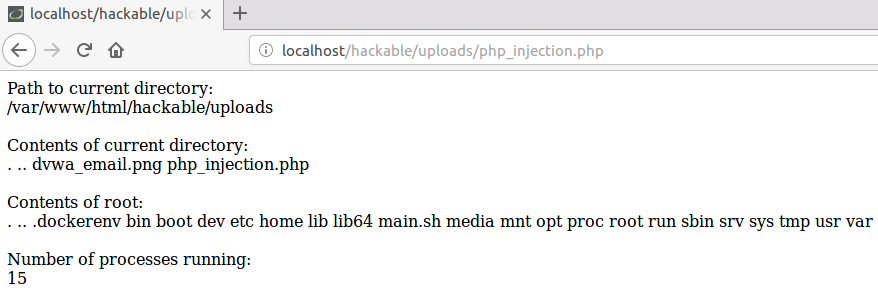
\includegraphics[width=.9\linewidth]{./php-injection.png}
  \caption{\label{fig:php-injection}
  Screenshot of the server's output after executing the PHP script}
\end{figure}

\noindent Observations:
\begin{itemize}
  \item When running \verb|ls /| on the server and the VM, there are a few notable differences. The server shows some hidden files
  such as \verb|.|, \verb|..|, and \verb|.dockerenv|, while the VM does not. However, the VM displays some files and directories that the server doesn't such as
  \verb|cdrom/|, \verb|initrd.img|, \verb|initrd.img.old|, \verb|lost+found/|, \verb|core/|, \verb|snap/|, \verb|vmlinuz|, \verb|vmlinuz.old|.
  \item Running \verb=ps aux --no-headers | wc -l= from the VM's terminal resulted in 226 processes instead of the 15 processes when running the command on the server.
  \item These differences stem from the way Docker creates and manages containers. Docker uses cgroups to manage resource allocation
  and isolates the container's processes from the host machine through the use of namespaces.
  Each container also has its own root file system, which explains the different views of the filesystem when running \verb|ls /|.~\cite{codementor,demystify}
\end{itemize}

\subsubsection*{Content Security Bypass}
On the CSP Bypass page, there is an input that allows external scripts from certain allowed sites
to be run. To execute Javascript that creates a popup alert, the following line of JavaScript was inserted into pastebin:
\begin{minted}{javascript}
  alert("content security policy bypass");
\end{minted}
Then, the pastebin link to the raw text (\verb|https://pastebin.com/raw/xkPZCMcs|) was pasted into the CSP Bypass page's input box and the include button was pressed.
The following figure displays the result when the server executed the script:
\begin{figure}[htbp]
  \centering
  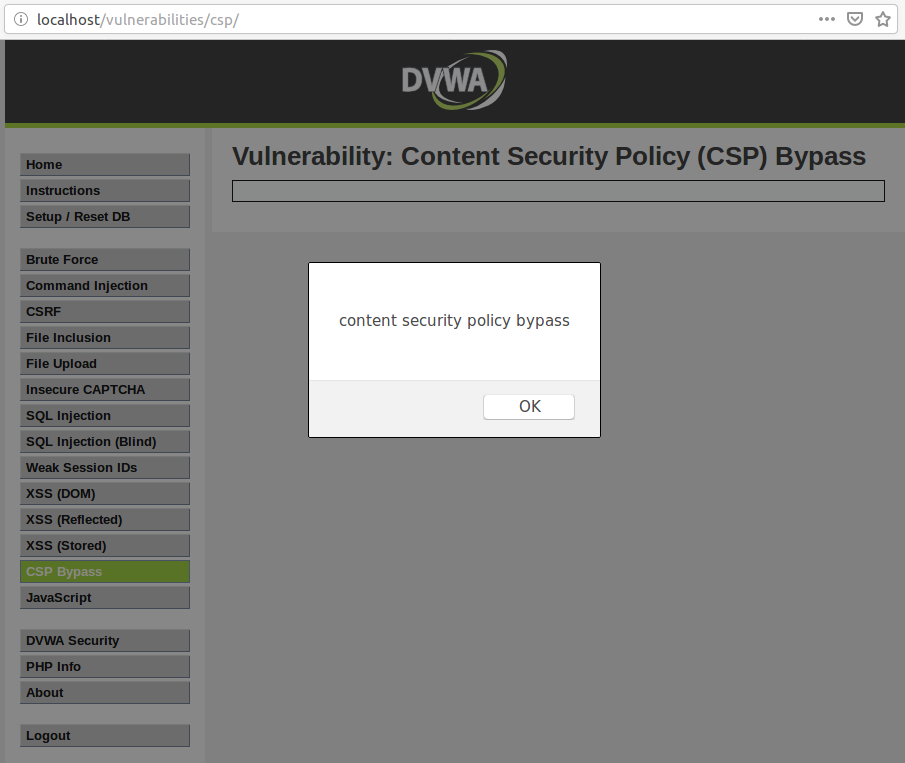
\includegraphics[width=.9\linewidth]{./csp.png}
  \caption{\label{fig:csp}
  Screenshot of the popup window generated by the JavaScript script injected through the CSP vulnerability}
\end{figure}

\subsubsection*{SQL Injection}
The objective of this section was to extract the username and password of every user account in the database
through a SQL Injection attack on the SQL Injection tab.
The simplest vulnerability to test for is if the developer concatenated the input directly into a SQL query without sanitization like so:
\begin{minted}{javascript}
  query = "SELECT * FROM table_name WHERE column_name = '" + input_string + "';"
\end{minted}
If so,
\begin{verbatim}
  ' OR '1'='1
\end{verbatim}
would return all rows of the table, which it did as shown in Figure~\ref{fig:sql-1}.
Since the input string was not sanitized before using it to build SQL queries,
attackers can simply inject SQL queries to obtain information from the database.
The next step is to obtain the name of the table that stores all of the users.
The injection
\begin{verbatim}
  ' AND 1=1 UNION SELECT null,
    table_name FROM INFORMATION_SCHEMA.tables #
\end{verbatim}
extracted information about all of the table names in the database, as shown in Figure~\ref{fig:sql-2}.
The \verb|#| at the end of the injection string starts an inline comment so that the server ignores the rest of the SQL query string.
The \verb|users| table seemed like the table that would contain the username and password for each user.
The last SQL injection
\begin{verbatim}
  ' AND 1=1 UNION SELECT user, password from users #
\end{verbatim}
successfully returned the username and hashed password of the users in the database (shown in Figure~\ref{fig:sql-3}.
\begin{figure}[htbp]
  \centering
  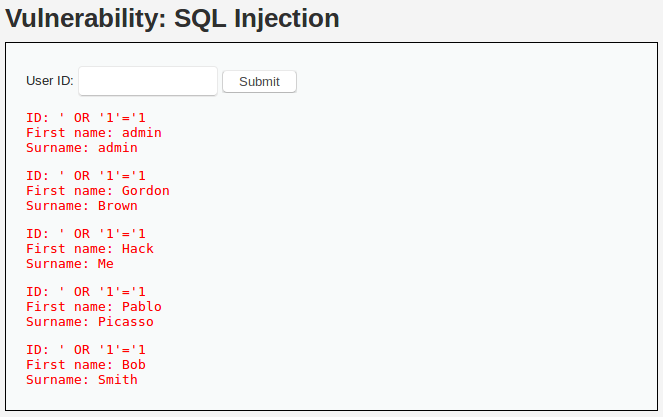
\includegraphics[width=1\linewidth]{./sql-1.png}
  \caption{\label{fig:sql-1}
  First SQL injection to check for a common SQL vulnerability}
\end{figure}
\begin{figure}[htbp]
  \centering
  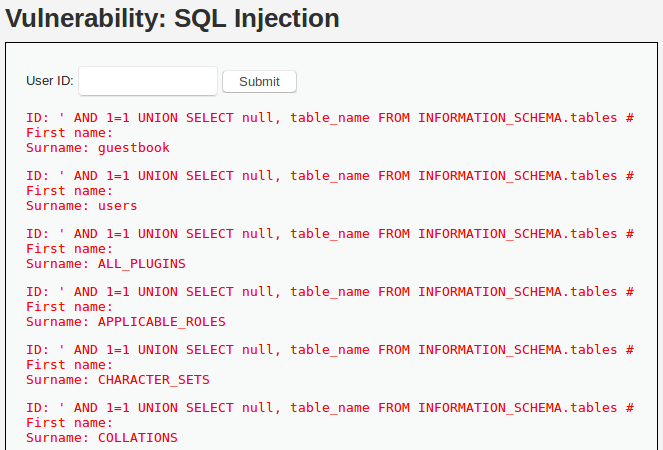
\includegraphics[width=1\linewidth]{./sql-2.png}
  \caption{\label{fig:sql-2}
  Result of query for all table names (not all results shown)}
\end{figure}
\begin{figure}[htbp]
  \centering
  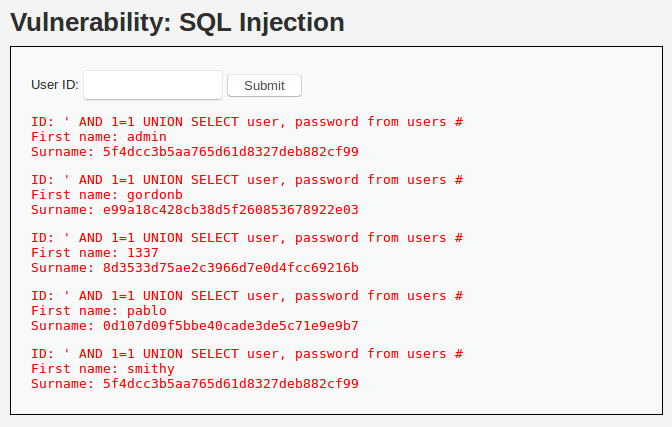
\includegraphics[width=1\linewidth]{./sql-3.png}
  \caption{\label{fig:sql-3}
  Result of query that selected the user and password from the users table}
\end{figure}
The decrypted passwords were then decrypted using a website~\cite{md5}, as shown in Table~\ref{table:creds}.
\begin{table}[h]
  \centering
  \begin{tabular}{ |c|c|c|c|c|c| }
    \hline
    \textbf{USER:} & admin    & gordonb & 1337    & pablo   & smithy   \\ \hline
    \textbf{PASS:} & password & abc123  & charley & letmein & password \\ \hline
  \end{tabular}
  \caption{\label{table:creds}
  Table of credentials}
\end{table}

Containerizing the web app limited what the attack surface by isolating the web app from the host machine as shown through the PHP injection.
However, if the web app has vulnerabilities, containerizing the web app doesn't prevent attacks like Content Security Policy bypass and SQL injections,
since these vulnerabilities stem from the actual source code.
In conclusion, the container itself is still vulnerable to attacks, but the host machine is protected from attacks that occur inside the container.

\subsection*{1b - Getting familiar with strace}
In order to detect a DVWA exploit, a tool called \verb|strace| was used to log all the system calls made by the container.
This can be done by attaching \verb|strace| to the process called \verb|containerd|, which executes the system calls on behalf of the Docker container.
To attach \verb|strace| to \verb|containerd|, the PID of \verb|containerd| must be passed as an argument to \verb|strace|.
\noindent To get the PID of \verb|containerd|, the following command was run in the terminal:
\begin{minted}{bash}
  $ ps -ef | grep containerd
  root      1155     1  0 09:36 ?        00:00:08 /usr/bin/containerd
\end{minted}
\noindent Then to monitor the system calls made by DVWA run the following command:
\begin{minted}{bash}
  $ sudo strace -p 1155 -o strace.txt -f
\end{minted}
\noindent Then run DVWA in a different terminal window:
\begin{minted}{bash}
  $ docker run --rm -it -p 80:80 vulnerables/web-dvwa
\end{minted}

\noindent For demonstration purposes, a bash command was injected into the input in the 'Command Injection' tab:
\begin{minted}{bash}
  ; echo "malware" > /tmp/maliciousfile
\end{minted}

\noindent The semi colon closes off the \verb|ping| command making the server run the bash command that follows.
The following lines identify the malicious sytem calls made during the exploit:
\begin{minted}{bash}
  28552 execve("/bin/sh", ["sh", "-c", "ping  -c 4 ; echo \"malware\" > /t"...], [/* 9 vars */] <unfinished ...>
  ...
  28552 open("/tmp/maliciousfile", O_WRONLY|O_CREAT|O_TRUNC, 0666) = 3
  28552 fcntl(1, F_DUPFD, 10)             = 10
  28552 close(1)                          = 0
  28552 fcntl(10, F_SETFD, FD_CLOEXEC)    = 0
  28552 dup2(3, 1)                        = 1
  28552 close(3)                          = 0
  28552 write(1, "malware\n", 8)          = 8
  28552 dup2(10, 1)                       = 1
  28552 close(10)                         = 0
  28552 exit_group(0)                     = ?
  28552 +++ exited with 0 +++
\end{minted}

\subsection*{1c - Limit who on the network can access the website using iptables}
To disable the existing firewall, \verb|firewalld| must be masked to prevent it from being started by other services and stopped so that the system uses
\verb|iptables|' rules. This was done using the following command:
\begin{minted}{bash}
  $ systemctl mask firewalld && systemctl stop firewalld
\end{minted}
The \verb|iptables| rules can be modified to only allow \verb|10.157.90.8| to connect to the web server.
The following command appends this rule to the iptables file.
\begin{minted}{bash}
  $ sudo iptables \
      -A INPUT \          # append to chain INPUT
      -p tcp \            # specify protocol
      --dport 80 \        # specify port
      ! -s 10.157.90.8 \  # for all BUT specified source
      -j DROP             # DROP
\end{minted}
Any connections not from the specified IP will now be dropped.
The new \verb|iptables| rules can be displayed using the following command:
\begin{minted}{bash}
  $ sudo iptables -S
\end{minted}

\section*{Part 2 - SELinux}
\label{sec:part-1}
\subsection*{Policy Modules}
For this part of the lab, a simple policy module was created, and the file contexts were applied to the files and directories.
Then running the \verb|simple| executable, created a file, \verb|simple.txt|, with the \verb|simple_var_t| type.
The following figure shows the output of running \verb|ls -Z|:
\begin{figure}[htbp]
  \centering
  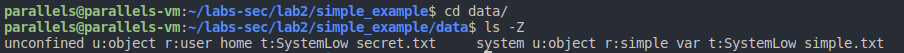
\includegraphics[width=.9\linewidth]{./ls-z.png}
  \caption{\label{fig:ls-z}
  Screenshot of the context of simple.txt}
\end{figure}

The following figure shows the error received when the \verb|simple| executable tries to read \verb|secret.txt| without the correct required permissions:
\begin{figure}[htbp]
  \centering
  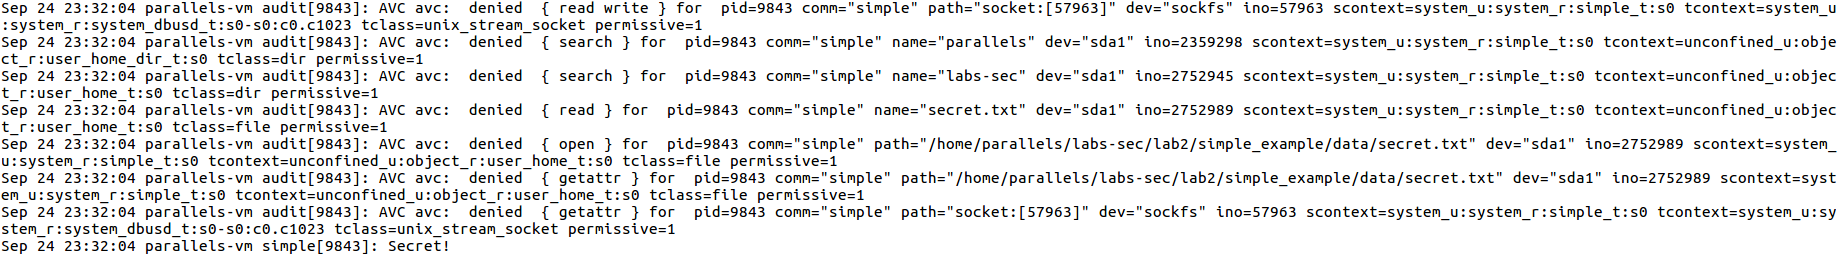
\includegraphics[width=.9\linewidth]{./log.png}
  \caption{\label{fig:log}
  Screenshot of log denying access to secret.txt}
\end{figure}

Context files (simple.fc) "declare the security contexts that are applied to files when the policy is installed"~\cite{context}.
Such security contexts include user, role, type, and level.
Type enforcement files (simple.te) define types and assign rules to each of the types.
Files associated with a specific type will have the permissions defined for that type.

\section*{Conclusion}
\label{sec:conclusion}
This lab was clearer than the previous lab, but still took quite a while to complete just this half.
This lab was pretty interesting and practical as it demonstrated some important concepts about containerization
as well as some common vulnerabilities and how to exploit them. Learning about these vulnerabilities also gave me a better understanding of
what to look out for when trying to write secure software.

\newpage
\nocite{*}
\bibliography{bibliography}
\bibliographystyle{ieeetr}
\end{document}
